\subsection{Neural Networks}

Neural networks is a model based on biology. 
Initially all neurons are connected. 
When the connection is used the connection becomes stronger and when they aren't used the connection becomes weaker.

The Stuttgart Neural Network Simulator is implemented in R in the RSNNS package.
The package can make a model of a artificial neural network (ANS) as a multi-layered perceptron.
% A lot of parameters can be specified but since the task is time demanding (see \ref{fig:neural_network_timing}) every option was not explored.
To reduce the inputs the data is normalized using the Z-Score method and a principle components analysis is made to give the most important data points.

\begin{figure}[h]
    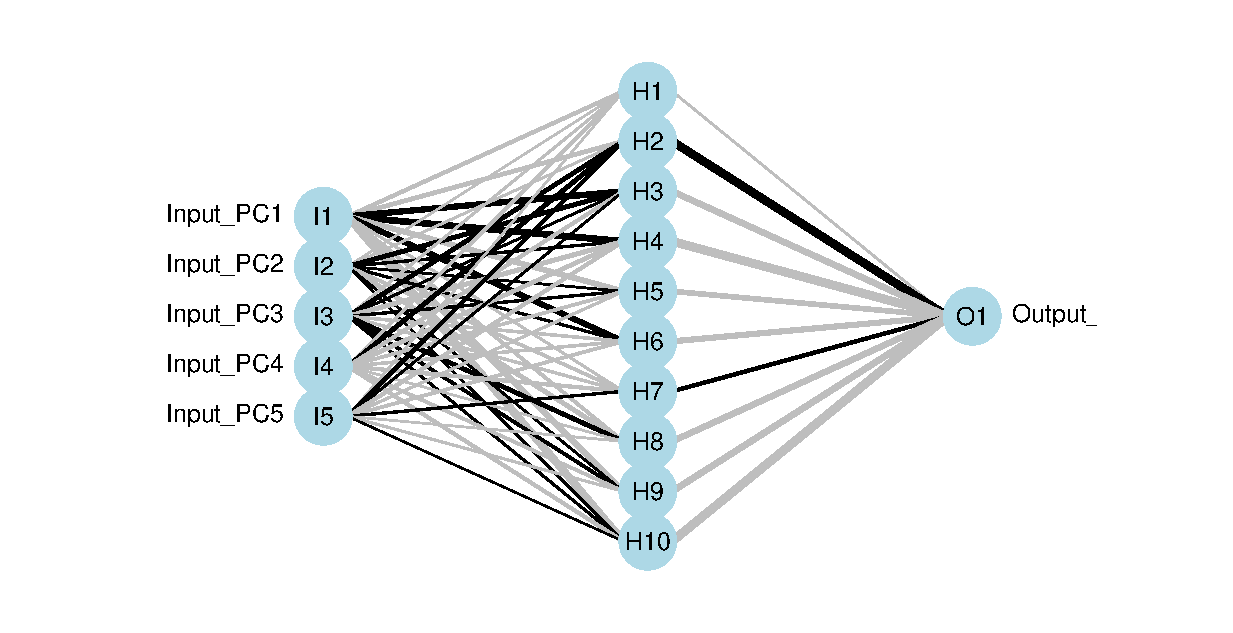
\includegraphics[width=\textwidth]{graphics/neural_network_visualized}
    \caption[Visualization of a neural network model.]{Visualization of a neural network model with 5 PC and 10 hidden layers. Plotted using \url{https://github.com/fawda123/NeuralNetTools}}
    \label{fig:neural_network_visualised}
\end{figure}

In the following section will the relationship with number of PC and the number of hidden layers be explored.
In figure \ref{fig:neural_network_visualised} is a small ANS shown.
It is important to notice that there is only a single output. 
Testing a digit will only show if the entered number resembles the train data or not.
In order to distinguish between multiple classes a model for each class is created.
Then the class with the highest resemblance is chosen.
The data is separated so it becomes 1 when the class matches and 0 when it doesn't.
To to determine the class of a test digit each model is tested as shown in code segment \ref{code:nn_separation}.

\lstinputlisting[language = R,
firstnumber = 36,
firstline = 36, 
lastline = 40, 
captionpos=b,
caption = {NN detection.},
label = {code:nn_separation}]{../Code/KNN/01/neural_network_simplified.R}

To investigate the relation between the number of PC and hidden layers both parameters were tested against each other in figure \ref{fig:contour_nn_size_vs_pca}. 
The problem tested is taking train data from all students and excluding the test person. 
The data is normalized with the z-score method.
From that it can be concluded that there is a sweet spot in the number of PC where the number of hidden layers is larger than the number of inputs.

\begin{figure}[h]
    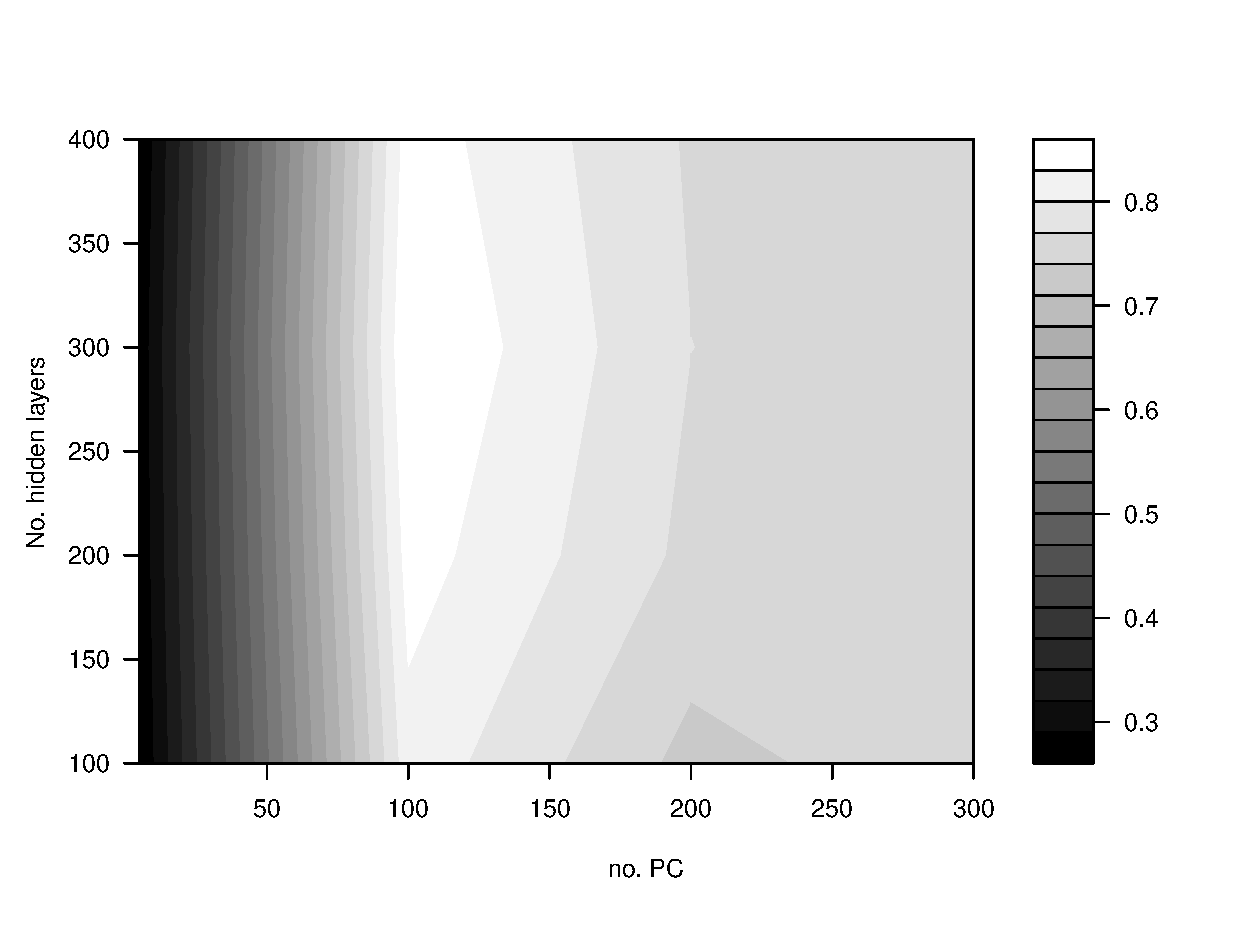
\includegraphics[width=\textwidth]{graphics/contour_nn_size_vs_pca}
    \caption[Success of neural network, PC vs HL]{Success of neural network when tested on G3M2 against everyone else's data.}
    \label{fig:contour_nn_size_vs_pca}
\end{figure}

The timing was measured in figure \ref{fig:contour_nn_both}.
The timing was split up into making the model and predicting the class.
The time it took to create the 10 models is shown in figure \ref{fig:contour_nn_size_vs_pca_time_model}.
% The time it took to predict all 4000 data points is shown in figure \ref{fig:contour_nn_size_vs_pca_time_predict}.
The biggest impact comes from number PC when building the model but the relationship is more linear when it comes to predicting.

\begin{figure}[h]
    \begin{subfigure}{0.49\textwidth}
    \centering
        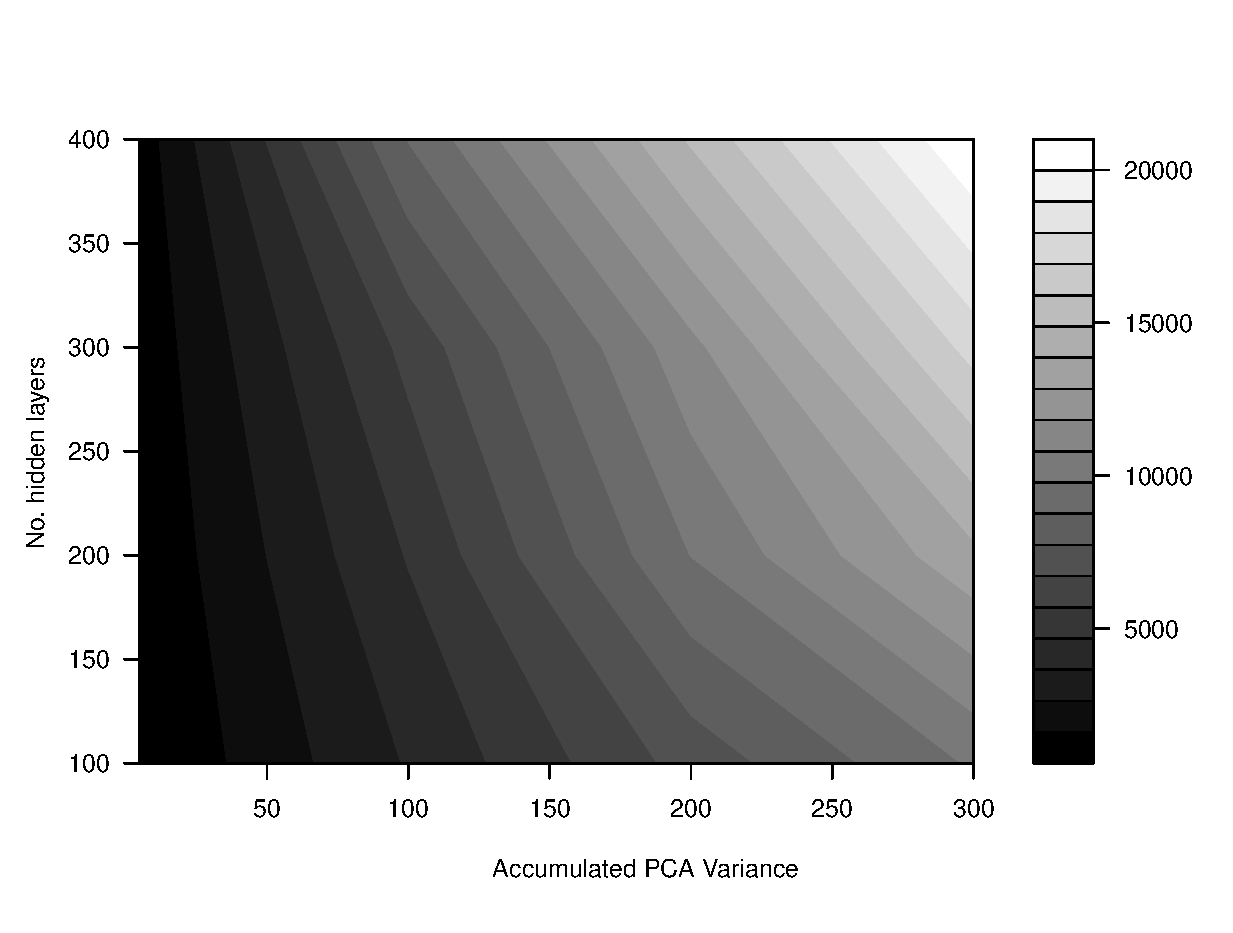
\includegraphics[width=\textwidth]{graphics/contour_nn_size_vs_pca_model}
        \caption{Time to build a neural network}
        \label{fig:contour_nn_size_vs_pca_time_model}
    \end{subfigure}
    \begin{subfigure}{0.49\textwidth}
        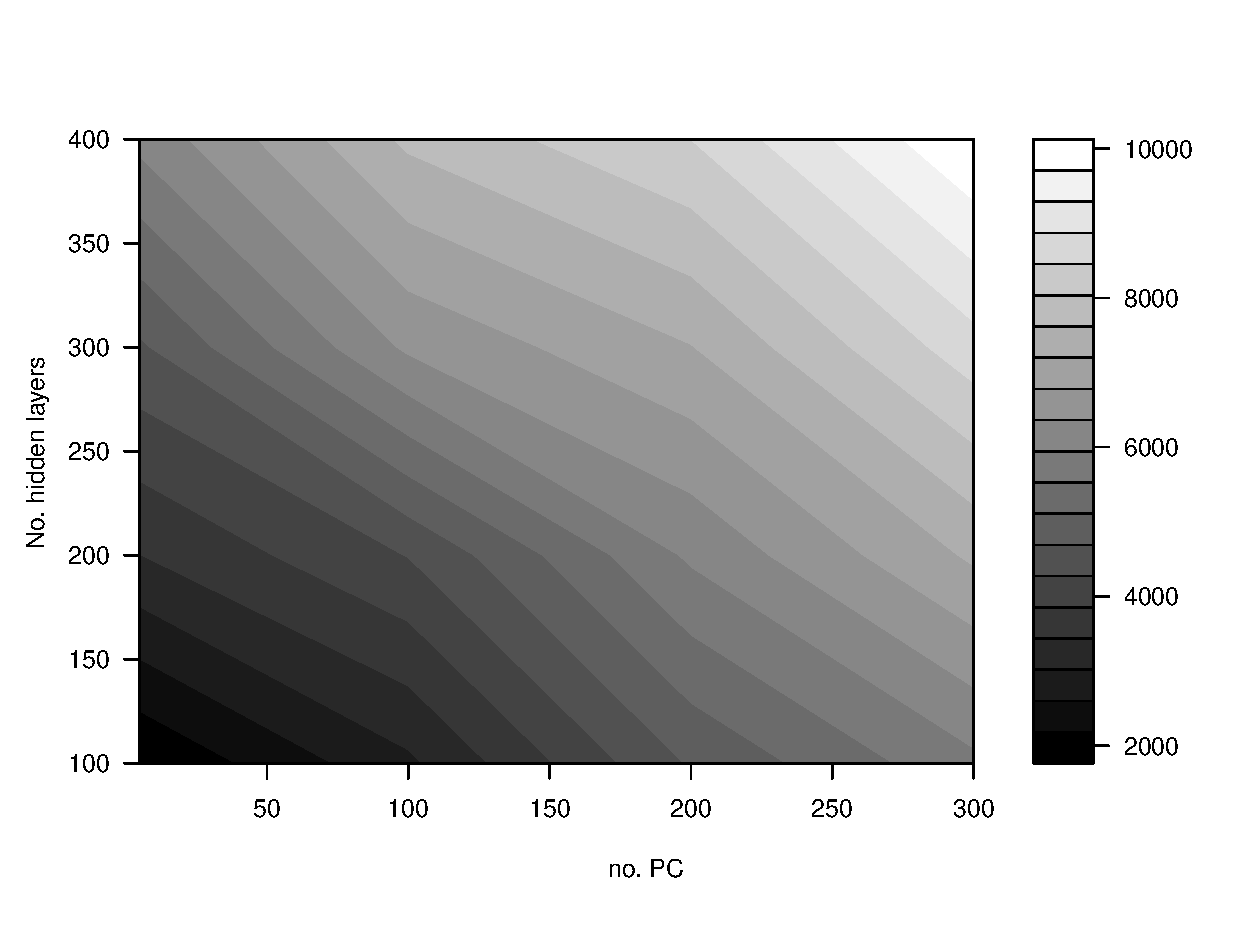
\includegraphics[width=\textwidth]{graphics/contour_nn_size_vs_pca_predict}
        \caption{Time of predicting using neural network}
        \label{fig:contour_nn_size_vs_pca_time_predict}
    \end{subfigure}
    \caption{Timing tested on G3M2 against everyone's data. The time is measured in seconds.}
    \label{fig:contour_nn_both}
\end{figure}

To view the impact of the train data size the timing and success was measured with a varying train set size.
The test is G3M2 tested against the rest of the students.
The data was normalized and the first 200 PC was used.
In all tests were 200 hidden layers in the neural network.
The Train size / digit refers to the number of samples per digit per person.
In figure \ref{fig:nn_timing_trainsize} is the timing and success plottet.
As expected is it shown that decreasing the train data will decrease the time it takes to build the model.
It is also shown that using more training digits does not increase the performance and thus this is a viable option.

\begin{figure}[h]
    \centering
    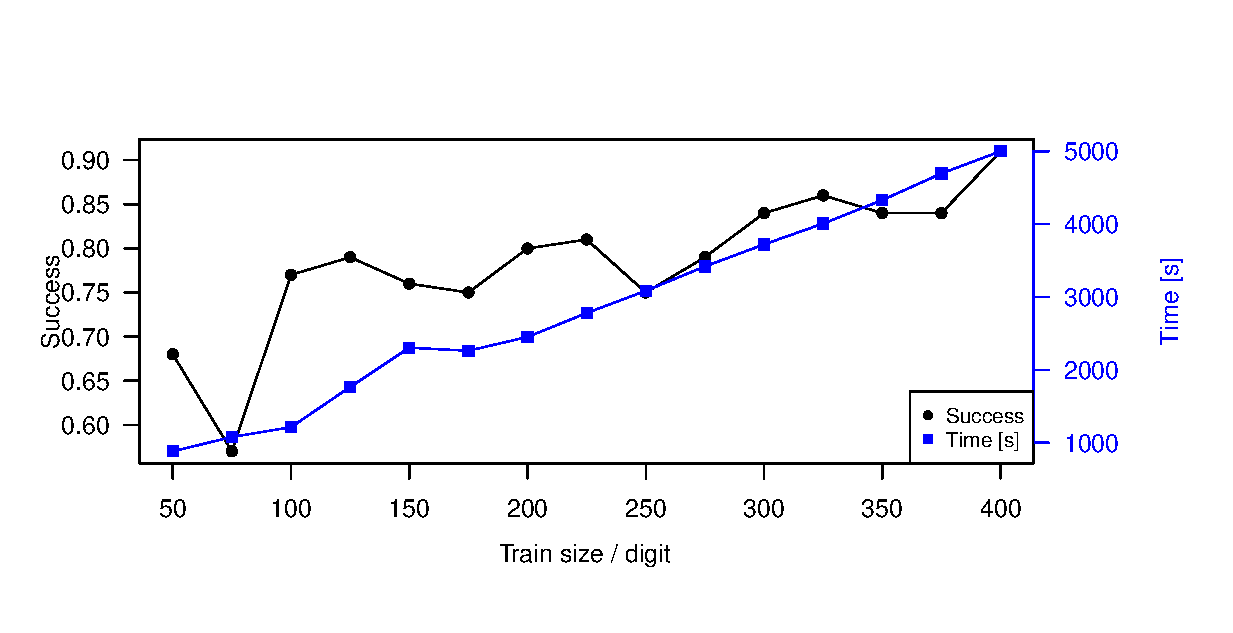
\includegraphics[width=\textwidth]{graphics/nn_timing_trainsize_200}
    \caption{Timing of building a neural network}
    \label{fig:nn_timing_trainsize}
\end{figure}
